\documentclass{beamer}
\usetheme{Boadilla}
\usecolortheme{seahorse}
\usefonttheme{serif}

\usepackage{lipsum}
\usepackage{graphicx,xcolor}
\usepackage{amsmath,amssymb,amsfonts}
% --- added for this project: diagrams, tables, theorem blocks, numbers generated from the experiments
\usepackage{tikz}
\usetikzlibrary{arrows.meta,positioning,calc,fit}
% styles that take a parameter must live outside frames (beamer reads frame bodies as macro arguments)
\tikzset{stage/.style={draw=#1, fill=#1!12, rounded corners=2pt, align=center, minimum height=10mm, inner sep=3pt}}
\tikzset{era/.style={draw=#1, fill=#1!7, rounded corners=3pt, text width=2.85cm, align=flush left, inner sep=4pt,
                     anchor=north, font=\scriptsize}}
\tikzset{tile/.style={draw=#1, fill=#1!9, rounded corners=3pt, text width=3.05cm, minimum height=1.75cm, align=center,
                      inner sep=3pt}}
\tikzset{road/.style={draw=#1, fill=#1!8, rounded corners=3pt, text width=3.15cm, align=flush left, inner sep=4pt,
                      anchor=north, font=\scriptsize}}
\usepackage{booktabs,array,multicol}
% generated by scripts/make_figures.py from results/metrics.json - do not edit
\newcommand{\EoneFreq}{0.00}
\newcommand{\EoneSTFT}{0.3}
\newcommand{\EoneLPC}{1.4}
\newcommand{\EthreeN}{4.25}
\newcommand{\EthreeRzero}{0.02}
\newcommand{\EfiveOne}{32}
\newcommand{\EfiveFive}{2.8}
\newcommand{\EfiveTen}{1.4}
\newcommand{\EsixTunedHidden}{96}
\newcommand{\EsixHiddenTwenty}{100}
\newcommand{\EthreeNnl}{4.42}
\newcommand{\EsixRandomHidden}{85}
\newcommand{\EsixFusedZero}{100}
\newcommand{\EsixAudioZero}{22}
\newcommand{\EsevenIdVision}{12.7}
\newcommand{\EsevenIdTap}{8.4}
\newcommand{\EsevenDiffVision}{68.2}
\newcommand{\EsevenDiffTap}{12.9}
\newcommand{\EfourClean}{0.007}
\newcommand{\EfourBlur}{0.009}
\newcommand{\EfourClear}{0.009}
\newcommand{\EeightR}{0.2}
\newcommand{\EeightRfar}{0.9}
\newcommand{\EeightH}{3}
\newcommand{\EeightCap}{4}
\newcommand{\EnineAvg}{375}
\newcommand{\EnineZero}{45}
\newcommand{\EnineTap}{7}
\newcommand{\EnineZeroSame}{12}
\newcommand{\EnineZeroTen}{171}
\newcommand{\EnineExp}{-2.01}
\newcommand{\EtenAbove}{1.2}
\newcommand{\EtenBelow}{14}


\definecolor{camc}{HTML}{2F6DB5}   % camera / vision
\definecolor{micc}{HTML}{C0392B}   % microphone / audio
\definecolor{phyc}{HTML}{C99A06}   % physics
\definecolor{fusc}{HTML}{2E8B57}   % fusion / outputs
\definecolor{watc}{HTML}{E8892B}   % water

\newtheorem{proposition}[theorem]{Proposition}
\newtheorem{law}[theorem]{Law}
\setbeamertemplate{theorems}[normal font]
\setbeamertemplate{navigation symbols}{}
\setbeamerfont{block title}{size=\small}   % 4:3 frames are tight: keep block titles on one line

% course-module tags: S = sound, V = images (vision), M = multimodal learning
\newcommand{\ctag}[2]{\tikz[baseline=-0.65ex]\node[fill=#1, text=white, circle, inner sep=0.7pt, font=\tiny\bfseries]{#2};}
\newcommand{\tagS}{\ctag{micc}{S}}
\newcommand{\tagV}{\ctag{camc}{V}}
\newcommand{\tagM}{\ctag{fusc}{M}}

% five probability bars at x-offset #1 in colour #2 (used in the fusion sketch)
\newcommand{\bars}[7]{\foreach \k/\h in {1/#3,2/#4,3/#5,4/#6,5/#7}{\fill[#2] ({#1+(\k-1)*0.27},0) rectangle ++(0.21,{\h*1.1});}}

\setbeamerfont{bibliography item}{size=\tiny}
\setbeamerfont{bibliography entry author}{size=\tiny}
\setbeamerfont{bibliography entry title}{size=\tiny}
\setbeamerfont{bibliography entry location}{size=\tiny}
\setbeamerfont{bibliography entry note}{size=\tiny}
\setbeamertemplate{bibliography item}{\insertbiblabel}
\let\oldthebibliography\thebibliography
\renewcommand{\thebibliography}[1]{\oldthebibliography{#1}\setlength{\itemsep}{1pt}\setlength{\parskip}{0pt}%
    \def\newblock{\hskip .11em plus .33em minus .07em}}

\title[TuneSight]{TuneSight: Seeing the Note, Hearing the Water}
\subtitle{DA321 Presentation: Physics-Guided Audio-Visual Fusion for a Self-Tuning Jal Tarang}
\author[Kushagra, 240150046]{Kushagra Singhal (240150046)}
\institute[DSAI, IITG]{Mehta Family School of Data Science and Artificial Intelligence\\Indian Institute of Technology, Guwahati}
\date{November 2026}
\titlegraphic{
\includegraphics[width=2cm]{images/logo/IITG.png}}

\begin{document}

\begin{frame}
\titlepage
\end{frame}


% Structure follows the course's suggested outline:
% title | motivation | past and current work | key highlights | what I learned | reflections | references
\section{Motivation and history}
% ------------------------------------------------------------------ slide 2
\begin{frame}{Motivation: a jal tarang that sees and listens}
        \centering
        \resizebox{0.78\linewidth}{!}{%
        \begin{tikzpicture}[font=\scriptsize, >={Stealth[length=2mm]}]
            \fill[gray!12] (-0.3,-0.25) rectangle (8.3,0);
            \foreach \i/\f in {0/0.85, 1/0.72, 2/0.58, 3/0.42, 4/0.24} {
                \pgfmathsetmacro{\x}{0.8+1.6*\i}
                \fill[watc!75] ({\x-0.42},0.06) -- ({\x+0.42},0.06) -- ({\x+0.42+0.12*\f},{0.06+1.6*\f}) -- ({\x-0.42-0.12*\f},{0.06+1.6*\f}) -- cycle;
                \draw[camc, line width=0.9pt] ({\x-0.45},0) -- ({\x+0.45},0) -- ({\x+0.57},1.75) -- ({\x-0.57},1.75) -- cycle;
            }
            \foreach \i/\n in {0/Sa, 1/Re, 2/Ga, 3/Pa, 4/Dha} { \node at ({0.8+1.6*\i},-0.5) {\n}; }
            % striker touching bowl 3
            \draw[brown!70!black, line width=2.2pt, line cap=round] (4.05,1.78) -- (5.3,3.0);
            \node[anchor=west] at (5.35,3.0) {striker};
            % camera
            \draw[camc, fill=camc!15, rounded corners=1pt] (-2.35,0.55) rectangle (-1.15,1.25);
            \draw[camc, fill=white] (-1.05,0.9) circle (0.16);
            \node[camc] at (-1.75,1.5) {camera};
            % microphone
            \draw[micc, fill=micc!15, rounded corners=3pt] (8.85,1.05) rectangle (9.25,1.75);
            \draw[micc] (9.05,1.05) -- (9.05,0.0);
            \node[micc] at (9.05,2.0) {mic};
            % laptop
            \node[draw, rounded corners=2pt, fill=fusc!10, draw=fusc, align=center] (pc) at (3.9,-1.55) {laptop: \textbf{TuneSight}};
            \draw[->, camc, thick] (-1.75,0.55) |- node[pos=0.75, below] {video: $h/H$, tip} (pc.west);
            \draw[->, micc, thick] (9.05,-0.0) |- node[pos=0.75, below] {audio: pitch $f$} (pc.east);
        \end{tikzpicture}}
    \vspace{3mm}
    \begin{columns}[T]
    \column{0.47\textwidth}
        \scriptsize
        \begin{itemize}
            \item The \textbf{jal tarang} is a row of bowls tuned with water: more water, lower pitch \cite{french1983}.
            \item \textbf{Q1.} Which of several \emph{identical} bowls was struck?
            \item \textbf{Q2.} How much water makes a bowl play a chosen swara?
        \end{itemize}
    \column{0.51\textwidth}
        \begin{block}{Idea}
            \scriptsize
            The camera sees the water (fill ratio $r = h/H$) but cannot hear; the microphone hears the pitch $f$ but cannot tell
            identical bowls apart. One physical law $f(r)$, \emph{learned online from a few taps}, joins them, so each modality
            predicts what the other should observe.
        \end{block}
    \end{columns}
\end{frame}

% ------------------------------------------------------------------ slide 3
\begin{frame}{Related work and what is new}
    \scriptsize
    \begin{tabular}{>{\raggedright\arraybackslash}p{0.46\linewidth} >{\raggedright\arraybackslash}p{0.46\linewidth}}
        \toprule
        \textbf{Already published} & \textbf{This project} \\
        \midrule
        Material recognition from image + impact sound \cite{gao2023objectfolder} &
            not claimed; only the modal (pole) model of sound is reused \\[2pt]
        Liquid level from the sound of \emph{pouring} \cite{liang2019pouringnet} &
            the \emph{struck} resonance + a physical law, taught by the camera \\[2pt]
        Sound-source localisation by appearance \cite{owens2016visually} &
            identical bowls defeat appearance; physics + striker motion \\[2pt]
        Jal tarang apps (virtual instruments) &
            tunes and transcribes a \emph{real} instrument \\
        \bottomrule
    \end{tabular}
    \vspace{2mm}
    \begin{exampleblock}{Contributions}
        \scriptsize
        \begin{enumerate}
            \item \textbf{Audio-visual correspondence for visually identical sources}, through a physical law instead of appearance.
            \item \textbf{Audio teaches vision}: online Bayesian calibration; model evidence recovers French's exponent $n\approx 4$ from data.
            \item \textbf{Vision-guided tuning} of a raga with one verification tap per bowl, and live sargam transcription.
        \end{enumerate}
    \end{exampleblock}
\end{frame}


\section{Key highlights}
% ------------------------------------------------------------------ key highlights at a glance
\begin{frame}{Key highlights at a glance}
    \label{sl:highlights}
    \centering
    \resizebox{\linewidth}{!}{%
    \begin{tikzpicture}[x=3.45cm, y=2.32cm]
        \node[tile=camc] at (0, 0) {{\Large\textbf{\textcolor{camc}{\EfiveFive\ cents}}}\\[3pt]
            \scriptsize camera-only pitch error after 5 taps: \emph{audio teaches vision}\\[2pt]{\tiny slide \pageref{sl:learning}}};
        \node[tile=phyc] at (1, 0) {{\Large\boldmath\textbf{\textcolor{phyc!75!black}{$n = \EthreeN$}}}\\[3pt]
            \scriptsize French's exponent, found by the data (theory: 4)\\[2pt]{\tiny slide \pageref{sl:learning}}};
        \node[tile=micc] at (2, 0) {{\Large\textbf{\textcolor{micc}{\EsixTunedHidden\,\%}}}\\[3pt]
            \scriptsize which of 5 identical bowls rang; striker hidden, 10~dB SNR\\[2pt]{\tiny slide \pageref{sl:results1}}};
        \node[tile=fusc] at (0, -1) {{\Large\textbf{\textcolor{fusc}{\EsixFusedZero{} vs \EsixAudioZero\,\%}}}\\[3pt]
            \scriptsize fused vs audio alone at 0~dB: two clues beat one\\[2pt]{\tiny slide \pageref{sl:results1}}};
        \node[tile=camc] at (1, -1) {{\Large\textbf{\textcolor{camc}{\EsevenIdTap\ cents}}}\\[3pt]
            \scriptsize tuning error for raga Bhupali after one check tap\\[2pt]{\tiny slide \pageref{sl:results2}}};
        \node[tile=gray] at (2, -1) {{\Large\textbf{\textcolor{gray!60!black}{No dataset}}}\\[3pt]
            \scriptsize one physical law, learned from a few taps\\[2pt]{\tiny slide \pageref{sl:physics}}};
    \end{tikzpicture}}
    \vspace{2mm}
    \begin{block}{What I built}
        \scriptsize
        A Python library (audio, vision, physics, fusion, tuning) $\cdot$ a live desktop app (webcam + mic, or simulated)
        $\cdot$ an interactive web explainer with ManimGL animations $\cdot$ experiments E1--E7 and 16 automated tests
        $\cdot$ code: \texttt{github.com/KUSHAGRA2606/TuneSight}
    \end{block}
\end{frame}

% ------------------------------------------------------------------ how it works: the big picture
\begin{frame}{How it works: two senses, one law}
    \label{sl:arch}
    \centering
    \resizebox{\linewidth}{!}{%
    \begin{tikzpicture}[font=\scriptsize, >={Stealth[length=2mm]}, line width=0.6pt,
        box/.style={draw, rounded corners=2pt, align=center, inner sep=3pt, minimum height=10mm, minimum width=20mm},
        cam/.style={box, draw=camc, fill=camc!10}, mic/.style={box, draw=micc, fill=micc!10},
        phy/.style={box, draw=phyc, fill=phyc!12, minimum width=28mm}, fus/.style={box, draw=fusc, fill=fusc!10, minimum width=28mm},
        outbox/.style={box, draw=fusc, fill=fusc!18, minimum height=7mm, minimum width=23mm},
        lab/.style={font=\tiny, inner sep=2.5pt}]
        \foreach \x/\t in {0/sensors, 3.0/what each sense measures, 7.3/reasoning, 11.6/outputs}
            \node[font=\tiny\itshape, text=gray] at (\x, 2.0) {\t};
        \node[cam] (camera) at (0, 1.15) {\textbf{Camera}\\video frames};
        \node[cam] (vision) at (3.0, 1.15) {\textbf{Vision}\\fill of each bowl,\\striker position};
        \node[mic] (micro) at (0, -1.15) {\textbf{Microphone}\\sound};
        \node[mic] (audio) at (3.0, -1.15) {\textbf{Audio}\\strike time,\\pitch};
        \node[phy] (phys) at (7.3, 1.15) {\textbf{The law}\\water level $\to$ pitch\\learned from taps};
        \node[fus] (fusion) at (7.3, -1.15) {\textbf{Fusion}\\sound $\times$ motion clue\\+ ``none of these''};
        \node[outbox] (tune) at (11.6, 1.15) {Tune to a raga};
        \node[outbox] (which) at (11.6, -0.7) {Which bowl?};
        \node[outbox] (sargam) at (11.6, -1.6) {Sargam notation};
        \draw[->, camc] (camera) -- (vision);
        \draw[->, micc] (micro) -- (audio);
        \draw[->, camc] (vision) -- node[lab, above] {fill ratio $r$} (phys);
        \draw[->, micc] (audio) -- node[lab, below] {pitch $f$} (fusion);
        \draw[->, camc, dashed] (vision.south east) -- node[lab, sloped, above, pos=0.45] {striker tip} (fusion.north west);
        \draw[->, phyc] ([xshift=6mm]phys.south) -- node[lab, right, align=left] {predicted pitch\\of every bowl} ([xshift=6mm]fusion.north);
        \draw[->, fusc] ([xshift=-6mm]fusion.north) -- node[lab, left] {learn} ([xshift=-6mm]phys.south);
        \draw[->, phyc] (phys) -- node[lab, above] {water level} (tune);
        \draw[->, fusc] (fusion.east) -- (which.west);
        \draw[->, fusc] (fusion.east) -- (sargam.west);
    \end{tikzpicture}}
    \vspace{1mm}
    \begin{block}{Every strike, in four steps}
        \scriptsize
        \textbf{1. Camera:} how full each bowl is just before the strike, and where the striker tip lands.\\
        \textbf{2. Microphone:} when the strike happened and what pitch it made.\\
        \textbf{3. Fusion:} compare the pitch with every bowl's \emph{predicted} pitch, add the striker clue, pick the bowl.\\
        \textbf{4. Learning:} the tap adds one (fill, pitch) point to the law, so the sound teaches the camera.
    \end{block}
\end{frame}

% ------------------------------------------------------------------ assumptions
\begin{frame}{The assumptions, and why they are reasonable}
    \label{sl:assumptions}
    \scriptsize
    \renewcommand{\arraystretch}{1.12}
    \begin{tabular}{@{}>{\raggedright\arraybackslash}p{0.335\linewidth} >{\raggedright\arraybackslash}p{0.30\linewidth} >{\raggedright\arraybackslash}p{0.30\linewidth}@{}}
        \toprule
        \textbf{Assumption} & \textbf{Why it is reasonable} & \textbf{If it fails} \\
        \midrule
        \textbf{A1.} Bowls are see-through; the water is coloured & the water line is visible by its colour & opaque bowls: look from the top \\
        \textbf{A2.} Same-shape bowls share one law & same glass, same physics \cite{french1983} & one check tap per bowl corrects it \\
        \textbf{A3.} Pitch = lowest strong ring, 150~Hz--8~kHz & the range of glass tumblers & a hum must also start at the strike and fade \\
        \textbf{A4.} One bowl is struck at a time & each sound has one source & needs multi-pitch analysis \\
        \textbf{A5.} The water is read just before the strike & then no hand hides it & use the last clear frames \\
        \textbf{A6.} The camera is fixed; bowls stay in place & each bowl keeps its identity & detect the bowls again \\
        \textbf{A7.} Camera and mic make independent errors & different sensors, different noise & fusion becomes over-confident \\
        \bottomrule
    \end{tabular}
    \vspace{2mm}
    \begin{block}{Why state them}
        \scriptsize
        Each assumption is a place where the system can fail. Naming it tells you what to check in a real setup,
        and it is exactly what the ``scope for improvement'' slide removes, one by one (slide \pageref{sl:improve}).
    \end{block}
\end{frame}

% ------------------------------------------------------------------ hearing
\begin{frame}{Hearing: from a tap to a pitch}
    \label{sl:hearing}
    \centering
    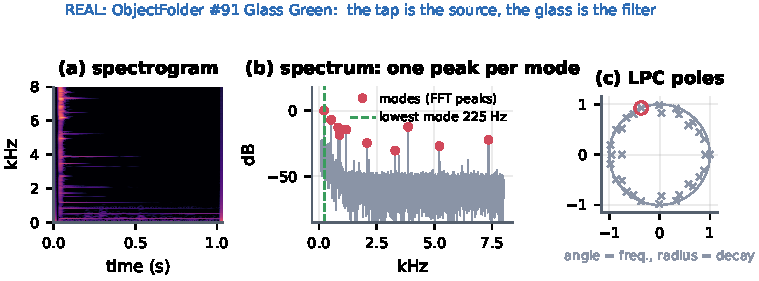
\includegraphics[width=0.80\linewidth]{images/figures/fig_strike.pdf}
    \vspace{-1mm}
    \begin{columns}[T]
    \column{0.47\textwidth}
        \begin{block}{The idea: a source and a filter}
            \scriptsize
            The tap is a short click (the \emph{source}). The bowl rings at a few fixed frequencies, its
            \emph{modes}, each fading like a bell (the \emph{filter}). It is the course's model of speech,
            applied to a bowl. The note we hear is the lowest strong mode.
        \end{block}
    \column{0.51\textwidth}
        \scriptsize
        \textbf{Steps}
        \begin{enumerate}
            \item Find the strike: a sudden jump in loudness.
            \item Spectrum (FFT): each peak is one mode (panel b).
            \item Keep a peak only if it \emph{starts at the strike and fades}: hum and fans are ignored.
            \item Pitch = the lowest strong peak.
            \item Cross-check: a second method (LPC, panel c) must find the same modes.
        \end{enumerate}
    \end{columns}
\end{frame}

% ------------------------------------------------------------------ seeing
\begin{frame}{Seeing: the water level from pixels}
    \label{sl:vision}
    \centering
    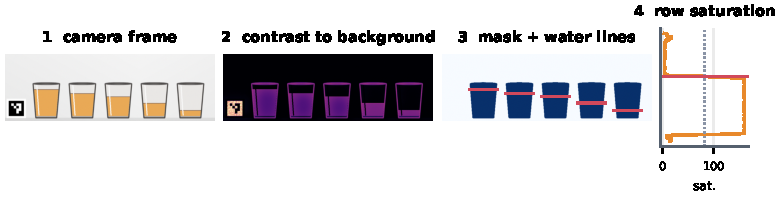
\includegraphics[width=0.96\linewidth]{images/figures/fig_vision_steps.pdf}
    \vspace{-1mm}
    \begin{columns}[T]
    \column{0.52\textwidth}
        \scriptsize
        \textbf{Steps}
        \begin{enumerate}
            \item \textbf{Background:} smooth away the bowls to see the empty, backlit scene.
            \item \textbf{Objects:} pixels darker than it, or coloured, are bowl or water; an automatic (Otsu) threshold
                  \cite{otsu1979threshold} sets ``darker''. One outline per bowl.
            \item \textbf{Water line:} going down a bowl, the row where colour appears (panel 4).
        \end{enumerate}
    \column{0.46\textwidth}
        \scriptsize
        \begin{enumerate}\setcounter{enumi}{3}
            \item \textbf{Fill ratio} $r = h/H$: water height over bowl height, so no camera scale is needed.
                  A printed marker \cite{garrido2014aruco} adds cm and ml.
            \item \textbf{Striker tip:} the lowest new pixel at the moment of the strike.
        \end{enumerate}
        \textbf{Why classical vision:} every step can be checked by eye, and it needs no training data.
    \end{columns}
\end{frame}

% ------------------------------------------------------------------ the law
\begin{frame}{The law that joins them: more water, lower pitch}
    \label{sl:physics}
    \begin{columns}[c]
    \column{0.55\textwidth}
        \begin{block}{French's law for a glass \cite{french1983}}
            \scriptsize
            \begin{minipage}[c]{0.33\linewidth}
                \centering
                \begin{tikzpicture}[scale=0.58, font=\tiny, >={Stealth[length=1.2mm]}]
                    \fill[watc!75] (-0.62,0.18) -- (0.62,0.18) -- (0.72,1.3) -- (-0.72,1.3) -- cycle;
                    \fill[gray!35] (-0.66,0) rectangle (0.66,0.18);
                    \draw[camc, line width=0.8pt] (-0.66,0) -- (0.66,0) -- (0.88,2.4) -- (-0.88,2.4) -- cycle;
                    \draw[<->] (1.2,0) -- (1.2,2.4) node[midway, right, inner sep=1pt] {$H$};
                    \draw[<->] (-1.1,0) -- (-1.1,1.3) node[midway, left, inner sep=1pt] {$h$};
                \end{tikzpicture}
            \end{minipage}\hfill
            \begin{minipage}[c]{0.65\linewidth}
                \[ f = \frac{f_0}{\sqrt{1 + \beta\, r^{\,n}}}, \qquad r = \frac{h}{H} \]
                \tiny
                $f_0$: pitch of the empty bowl\\
                $\beta$: how strongly water lowers it (one number per bowl type)\\
                $n = 4$ for a thin wall\\
                ($h$ is measured above the thick base)
            \end{minipage}
        \end{block}
        \begin{block}{The logic}
            \scriptsize
            Water touching the wall moves with it and adds mass, so the wall vibrates more slowly.
            A little water barely matters ($r^4$ is tiny); near the top the pitch drops fast (right, a).\\[2pt]
            Written as $1/f^2$ against $r^n$, the law is a \textbf{straight line} (right, b), so a few taps are enough to fit it.
        \end{block}
    \column{0.43\textwidth}
        \centering
        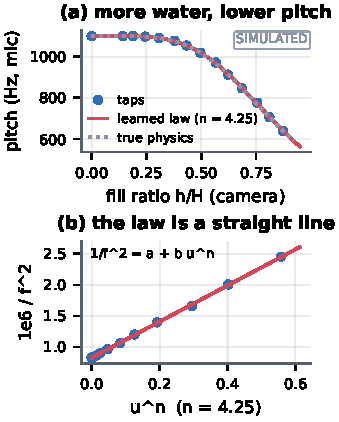
\includegraphics[width=\linewidth]{images/figures/fig_law_tall.pdf}
    \end{columns}
\end{frame}

% ------------------------------------------------------------------ learning from taps
\begin{frame}{Learning the law from taps: audio teaches vision}
    \label{sl:learning}
    \centering
    \resizebox{\linewidth}{!}{%
    \begin{tikzpicture}[font=\scriptsize, >={Stealth[length=2mm]}, node distance=5mm]
        \node[stage=gray] (tap) {\textbf{Tap}\\a bowl};
        \node[stage=gray, right=of tap] (meas) {\textcolor{camc}{camera: fill $r$}\\\textcolor{micc}{mic: pitch $f$}};
        \node[stage=phyc, right=of meas] (pt) {\textbf{one point}\\$(r, f)$};
        \node[stage=phyc, right=of pt] (fit) {\textbf{update}\\the line};
        \node[stage=fusc, right=of fit] (pred) {\textbf{camera alone}\\predicts pitch};
        \draw[->] (tap) -- (meas); \draw[->] (meas) -- (pt); \draw[->] (pt) -- (fit); \draw[->] (fit) -- (pred);
        \draw[->, gray] (pred.south) -- ++(0,-0.35) -| node[pos=0.25, below, font=\tiny] {next tap} (tap.south);
    \end{tikzpicture}}
    \vspace{1mm}
    \begin{columns}[T]
    \column{0.55\textwidth}
        \scriptsize
        \begin{itemize}
            \item \textbf{Start from physics:} a rough guess for $f_0$ and $\beta$, with wide uncertainty.
            \item \textbf{Each tap adds one point}; Bayesian linear regression \cite{bishop2006pattern} updates the straight line
                  \emph{and} says how sure it is.
            \item \textbf{The data choose $n$:} the best-supported exponent is $n = \EthreeN$ (theory 4).
            \item \textbf{Assumed noise:} pitch $\pm 8$ cents per tap; water level $\pm 0.6\,\%$ of the bowl.
        \end{itemize}
        \vspace{1mm}
        \textbf{Result:} after 5 taps the camera alone predicts any bowl's pitch within \textbf{\EfiveFive\ cents} (right).
    \column{0.43\textwidth}
        \centering
        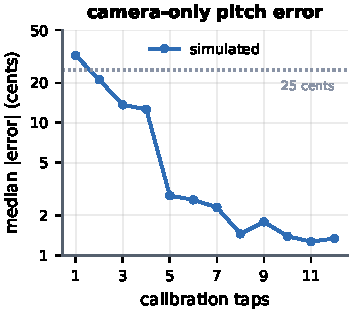
\includegraphics[width=\linewidth]{images/figures/fig_learning.pdf}
    \end{columns}
\end{frame}

% ------------------------------------------------------------------ fusion
\begin{frame}{Which bowl rang? Combining two clues}
    \label{sl:fusion}
    \begin{columns}[T]
    \column{0.54\textwidth}
        \scriptsize
        \begin{itemize}
            \item \textbf{Clue 1, sound:} the camera predicts each bowl's pitch from its water. The closer the heard pitch is
                  to a bowl's prediction, the higher that bowl scores (top right).
            \item \textbf{Clue 2, motion:} the striker tip lands on one bowl; nearby bowls score higher.
            \item \textbf{Combine:} multiply the two scores, trusting each clue by how reliable it is \emph{now}
                  \cite{ernst2002humans}: noisy sound $\Rightarrow$ trust motion; hidden striker $\Rightarrow$ trust sound.
            \item \textbf{Safety:} if no prediction fits the sound, the answer is ``none of these''.
        \end{itemize}
        \vspace{1mm}
        \textbf{Assumes} the two clues make independent errors (A7).
    \column{0.44\textwidth}
        \centering
        \resizebox{\linewidth}{!}{%
        \begin{tikzpicture}[font=\tiny, x=0.9cm, y=0.9cm]
            \draw[->] (0,0) -- (4.4,0) node[right] {pitch};
            \foreach \c/\lab in {0.6/1, 1.4/2, 2.2/3} {
                \pgfmathsetmacro{\lo}{\c-0.4}\pgfmathsetmacro{\hi}{\c+0.4}
                \draw[phyc, thick] plot[domain=\lo:\hi, samples=40] (\x,{0.9*exp(-((\x-\c)^2)/0.016)});
                \node[phyc] at (\c,1.02) {\lab};
            }
            \draw[phyc, thick] plot[domain=2.85:3.65, samples=40] (\x,{0.9*exp(-((\x-3.25)^2)/0.016)});
            \node[phyc, anchor=west] at (3.45,0.7) {4 and 5};
            \draw[micc, dashed, thick] (3.25,0) -- (3.25,1.05) node[above] {heard};
            \node at (2.1,-0.3) {predicted pitch of bowls 1--5 (from the camera)};
        \end{tikzpicture}}\\[2mm]
        \resizebox{\linewidth}{!}{%
        \begin{tikzpicture}[font=\scriptsize, x=1cm, y=1cm]
            \bars{0}{micc}{0.02}{0.02}{0.02}{0.47}{0.47}
            \bars{1.75}{camc}{0.02}{0.02}{0.03}{0.08}{0.85}
            \bars{3.5}{fusc}{0.0}{0.0}{0.0}{0.08}{0.92}
            \draw (-0.1,0) -- (4.9,0);
            \node at (1.52,0.5) {$\times$}; \node at (3.27,0.5) {$=$};
            \node[font=\tiny] at (0.645,-0.18) {sound}; \node[font=\tiny] at (2.395,-0.18) {motion}; \node[font=\tiny] at (4.145,-0.18) {combined};
            \node[font=\tiny, align=center] at (2.4,-0.62) {bowls 4 and 5 hold the same water:\\sound is 50/50, the striker's motion decides};
        \end{tikzpicture}}
    \end{columns}
\end{frame}

% ------------------------------------------------------------------ tuning
\begin{frame}{Tuning by sight: from a raga to millilitres}
    \label{sl:tuning}
    \begin{columns}[T]
    \column{0.53\textwidth}
        \scriptsize
        Raga Bhupali; each note is a fixed ratio of Sa:\\[1mm]
        \centerline{\begin{tabular}{@{}ccccc@{}}
            Sa & Re & Ga & Pa & Dha\\ \hline
            $1$ & $\tfrac98$ & $\tfrac54$ & $\tfrac32$ & $\tfrac53$
        \end{tabular}}
        \vspace{1mm}
        \begin{enumerate}
            \item \textbf{Pick Sa} so every note is reachable: water can only \emph{lower} a bowl's pitch.
            \item \textbf{Turn the law around:} note $\to$ water level $\to$ ml to pour (from the bowl's shape).
            \item \textbf{Stop one semitone early:} water is easy to add, hard to remove.
            \item \textbf{Tap once:} it shows how this bowl differs from the shared law; correct, then top up.
        \end{enumerate}
    \column{0.45\textwidth}
        \centering
        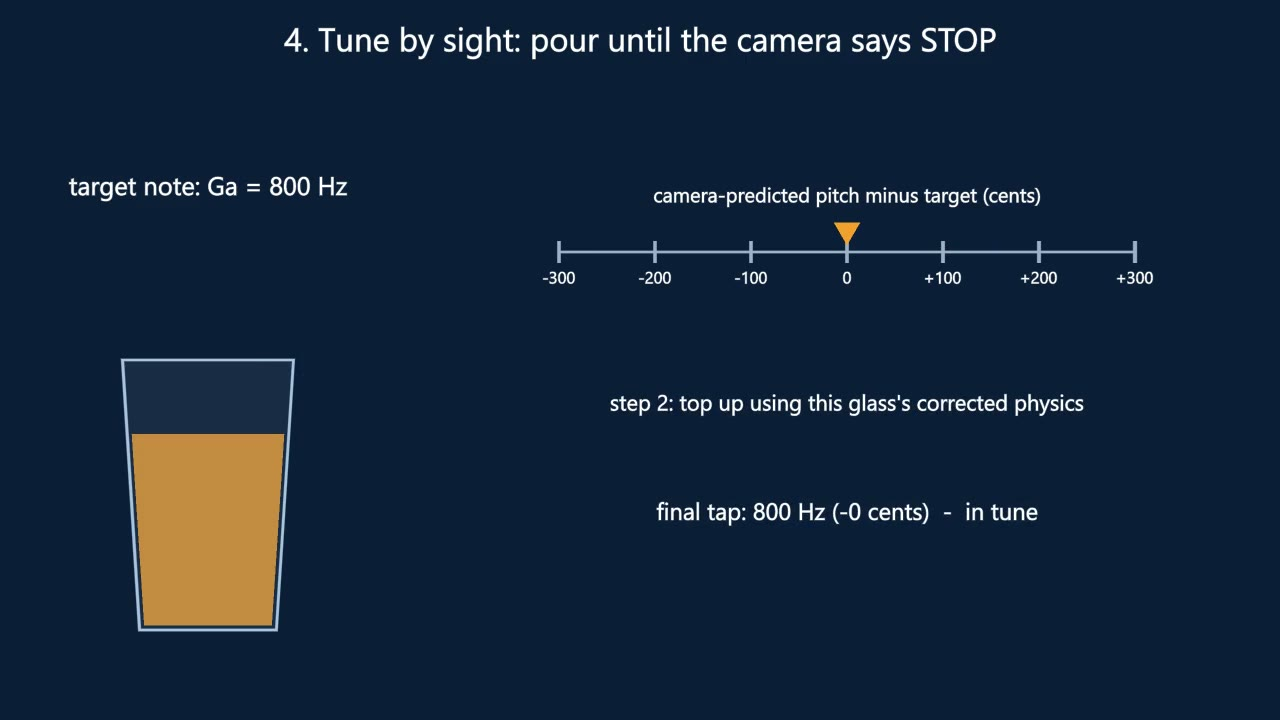
\includegraphics[width=\linewidth]{images/figures/anim_tune.jpg}\\[-0.5mm]
        {\tiny The camera's pitch gauge stops the pour; one tap fixes the last cents.\par}
    \end{columns}
    \vspace{2mm}
    \centering
    \resizebox{\linewidth}{!}{%
    \begin{tikzpicture}[font=\scriptsize, >={Stealth[length=2mm]}, node distance=4mm]
        \node[stage=camc] (plan) {\textbf{Plan}\\Sa, water levels};
        \node[stage=camc, right=of plan] (pour) {\textbf{Pour}\\camera tracks the level};
        \node[stage=phyc, right=of pour] (stop) {\textbf{Stop early}\\one semitone sharp};
        \node[stage=micc, right=of stop] (tap) {\textbf{Tap}\\measure the offset};
        \node[stage=camc, right=of tap] (top) {\textbf{Top up}\\corrected target};
        \node[stage=fusc, right=of top] (ok) {\textbf{Verify}\\tap: error in cents};
        \draw[->] (plan) -- (pour); \draw[->] (pour) -- (stop); \draw[->] (stop) -- (tap); \draw[->] (tap) -- (top); \draw[->] (top) -- (ok);
        \draw[->, gray] (ok.south) -- ++(0,-0.3) -| node[pos=0.25, below, font=\tiny] {next bowl} (pour.south);
    \end{tikzpicture}}
\end{frame}

% ------------------------------------------------------------------ beyond identical glasses
\begin{frame}{Beyond identical glasses: new shapes and opaque cups}
    \label{sl:general}
    \begin{columns}[T]
    \column{0.49\textwidth}
        \centering
        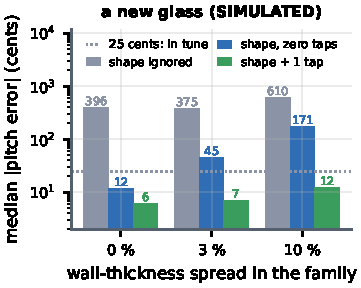
\includegraphics[width=\linewidth]{images/figures/fig_newcontainer.pdf}
    \column{0.49\textwidth}
        \centering
        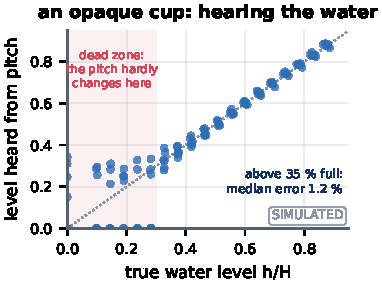
\includegraphics[width=\linewidth]{images/figures/fig_hearlevel.pdf}
    \end{columns}
    \vspace{1mm}
    \scriptsize
    \begin{itemize}
        \item \textbf{A new glass} (left): ignoring its shape, the pitch is \EnineAvg\ cents off; its shape alone gives \EnineZero\ cents
              (\EnineZeroSame\ if all walls are equal); one check tap gives \EnineTap. The hidden wall thickness sets the limit.
        \item \textbf{An opaque cup} (right): one tap when empty, then each tap's pitch gives the level, within \EtenAbove\,\% of the
              height above 35\,\% full. Below 30\,\% the law is too flat: a tap varies more (8 cents) than the water changes it.
        \item The fitted radius exponent is $\EnineExp$, close to French's $-2$: the camera and the taps recover the physics.
    \end{itemize}
\end{frame}


\section{Learning and reflections}
% ------------------------------------------------------------------ what I learned (1): course concepts
\begin{frame}{What I learned (1): course concepts at work}
    \label{sl:concepts}
    \scriptsize
    \renewcommand{\arraystretch}{1.08}
    \begin{tabular}{@{}c >{\raggedright\arraybackslash}p{0.345\linewidth} >{\raggedright\arraybackslash}p{0.465\linewidth} c@{}}
        \toprule
        & \textbf{Course concept} & \textbf{How TuneSight uses it} & \textbf{Slide}\\
        \midrule
        \tagS & Sampling, DFT/FFT, windowing, STFT & the ring frequencies (modes) of each strike, and how fast each fades & \pageref{sl:hearing}\\
        \tagS & LTI systems, impulse response, linear prediction, source--filter model & the tap is the source, the bowl the filter; LPC cross-checks the modes & \pageref{sl:hearing}\\
        \tagV & Thresholding (Otsu), morphology, contours & bowl silhouettes from a backlit frame & \pageref{sl:vision}\\
        \tagV & Colour spaces (HSV), intensity profiles & the water line from row saturation (edge step for clear water) & \pageref{sl:vision}\\
        \tagV & Camera geometry, fiducial markers & centimetres and millilitres from an ArUco marker & \pageref{sl:vision}\\
        \tagM & Regression, Bayesian inference, model evidence & learning the law online, and choosing its exponent & \pageref{sl:learning}\\
        \tagM & Multisensory integration, cue reliability, inverse effectiveness & weighted fusion of audio and striker motion, plus a ``none'' check & \pageref{sl:fusion}\\
        \bottomrule
    \end{tabular}
    \vspace{2mm}
    \begin{block}{What joining them taught me}
        \scriptsize
        One physical law ties the course topics together: audio \emph{labels} vision (fill $\to$ pitch), and fusion
        weighs each sense strike by strike. \hfill {\tiny\tagS{} sound \ \tagV{} images \ \tagM{} multimodal}
    \end{block}
\end{frame}

% ------------------------------------------------------------------ what I learned (2): lessons
\begin{frame}{What I learned (2): lessons beyond the formulas}
    \label{sl:lessons}
    \centering
    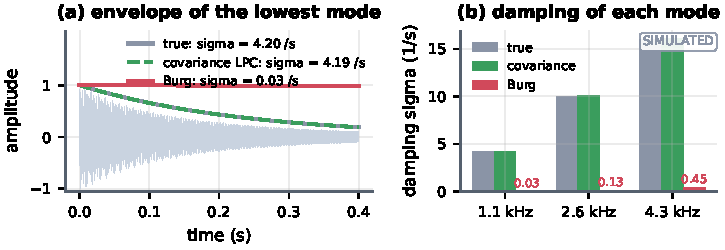
\includegraphics[width=0.76\linewidth]{images/figures/fig_burg.pdf}\\[-0.5mm]
    {\tiny Lesson 2 in one picture: on a decaying ring Burg's method finds almost no damping; the covariance method is exact.\par}
    \vspace{1.5mm}
    \begin{columns}[T]
    \column{0.5\textwidth}
        \scriptsize
        \begin{enumerate}
            \item \textbf{A law beats a dataset.} With the right physics, 5 taps give \EfiveFive~cents; a black box would need many labelled strikes.
            \item \textbf{Check a method's assumptions.} The textbook method (Burg \cite{burg1975maximum}) assumes a sound that does
                  not fade; a ringing bowl fades, so it got the fading 99\,\% wrong. A method without that assumption \cite{kumaresan1982estimating} is exact.
        \end{enumerate}
    \column{0.48\textwidth}
        \scriptsize
        \begin{enumerate}\setcounter{enumi}{2}
            \item \textbf{Fusion pays where a sense is weak:} at 0~dB, audio alone \EsixAudioZero\,\%, fused \EsixFusedZero\,\%.
            \item \textbf{Two clocks, one event:} align video to the audio onset; read the water \emph{before} the strike, when no hand hides it.
            \item \textbf{Simulate with ground truth first:} every module was tested against known answers before real data.
        \end{enumerate}
    \end{columns}
\end{frame}

% ------------------------------------------------------------------ reflections (a): surprises
\begin{frame}{Reflections (a): what surprised me}
    \label{sl:surprised}
    \begin{columns}[T]
    \column{0.39\textwidth}
        \centering
        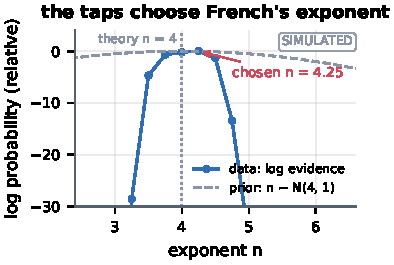
\includegraphics[width=0.96\linewidth]{images/figures/fig_evidence.pdf}
    \column{0.59\textwidth}
        \scriptsize
        \begin{itemize}
            \item \textbf{The data found the physics:} model evidence chose $n = \EthreeN$, French's exponent, with no tuning (left).
            \item \textbf{The textbook estimator failed:} Burg's method found almost no damping (slide \pageref{sl:lessons}).
            \item \textbf{Motion pointed at the wrong bowl:} the stick's body sweeps over the neighbour; only its tip is reliable.
            \item \textbf{``Identical'' is not identical:} a 3\,\% shape spread costs \EsevenDiffVision~cents; one tap brings it to \EsevenDiffTap.
        \end{itemize}
    \end{columns}
    \vspace{1mm}
    \centering
    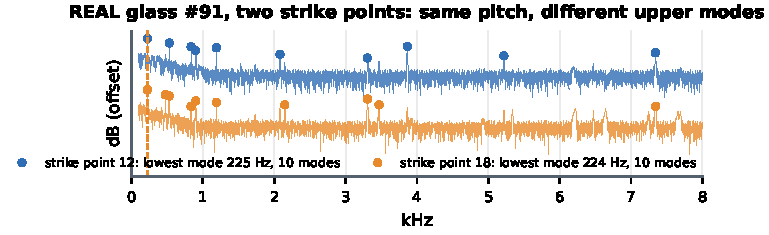
\includegraphics[width=0.80\linewidth]{images/figures/fig_strikepoint.pdf}\\[-0.5mm]
    {\tiny A real glass: the strike point changes the upper modes, not the lowest one (225 vs 224~Hz). One recording also has a 79~Hz line
    from the stand or room, 6~dB below the glass: searching from 60~Hz, it is taken as the pitch. A sensible band matters.\par}
\end{frame}

% ------------------------------------------------------------------ reflections (b): scope for improvement
\begin{frame}{Reflections (b): scope for improvement}
    \label{sl:improve}
    \centering
    \resizebox{\linewidth}{!}{%
    \begin{tikzpicture}[>={Stealth[length=2.5mm]}]
        \node[road=fusc] (r1) at (0, 0) {\textcolor{fusc}{\textbf{Next: real data}}\\[4pt]
            $\bullet$ Record a full session with real bowls and a musician\\[3pt]
            $\bullet$ Ruler check of the water line; real calibration and tuning results\\[3pt]
            $\bullet$ Mesh data for the size-scaling experiment (E2)};
        \node[road=camc] (r2) at (3.75, 0) {\textcolor{camc}{\textbf{Then: harder scenes}}\\[4pt]
            $\bullet$ Opaque porcelain bowls, as in a traditional jal tarang: a top-view or depth camera\\[3pt]
            $\bullet$ Two strikers and overlapping notes: multi-pitch analysis\\[3pt]
            $\bullet$ Reflections: a small learned water-line detector with the physics as its prior};
        \node[road=phyc] (r3) at (7.5, 0) {\textcolor{phyc!75!black}{\textbf{Later: beyond music}}\\[4pt]
            $\bullet$ Closed-loop tuning with a small pump\\[3pt]
            $\bullet$ A phone app: camera and mic in one device\\[3pt]
            $\bullet$ ``Tap and look'' level checks for rows of identical containers (bottles, tanks)};
        \foreach \x in {0, 3.75} \draw[->, thick, gray] (\x + 1.73, -1.0) -- (\x + 2.02, -1.0);
    \end{tikzpicture}}
    \vspace{2mm}
    \begin{alertblock}{Honest limitations today}
        \scriptsize
        Most results are simulated with known ground truth; the real audio is two ObjectFolder strikes of one glass.
        LPC damping degrades quickly with noise (1.4\,\% error at 40~dB, 54\,\% at 20~dB), and clear water needs the weaker edge cue.
    \end{alertblock}
\end{frame}

% ------------------------------------------------------------------ live demo and conclusion
\begin{frame}{Live demo and conclusion}
    \label{sl:demo}
    \begin{columns}[T]
    \column{0.54\textwidth}
        \centering
        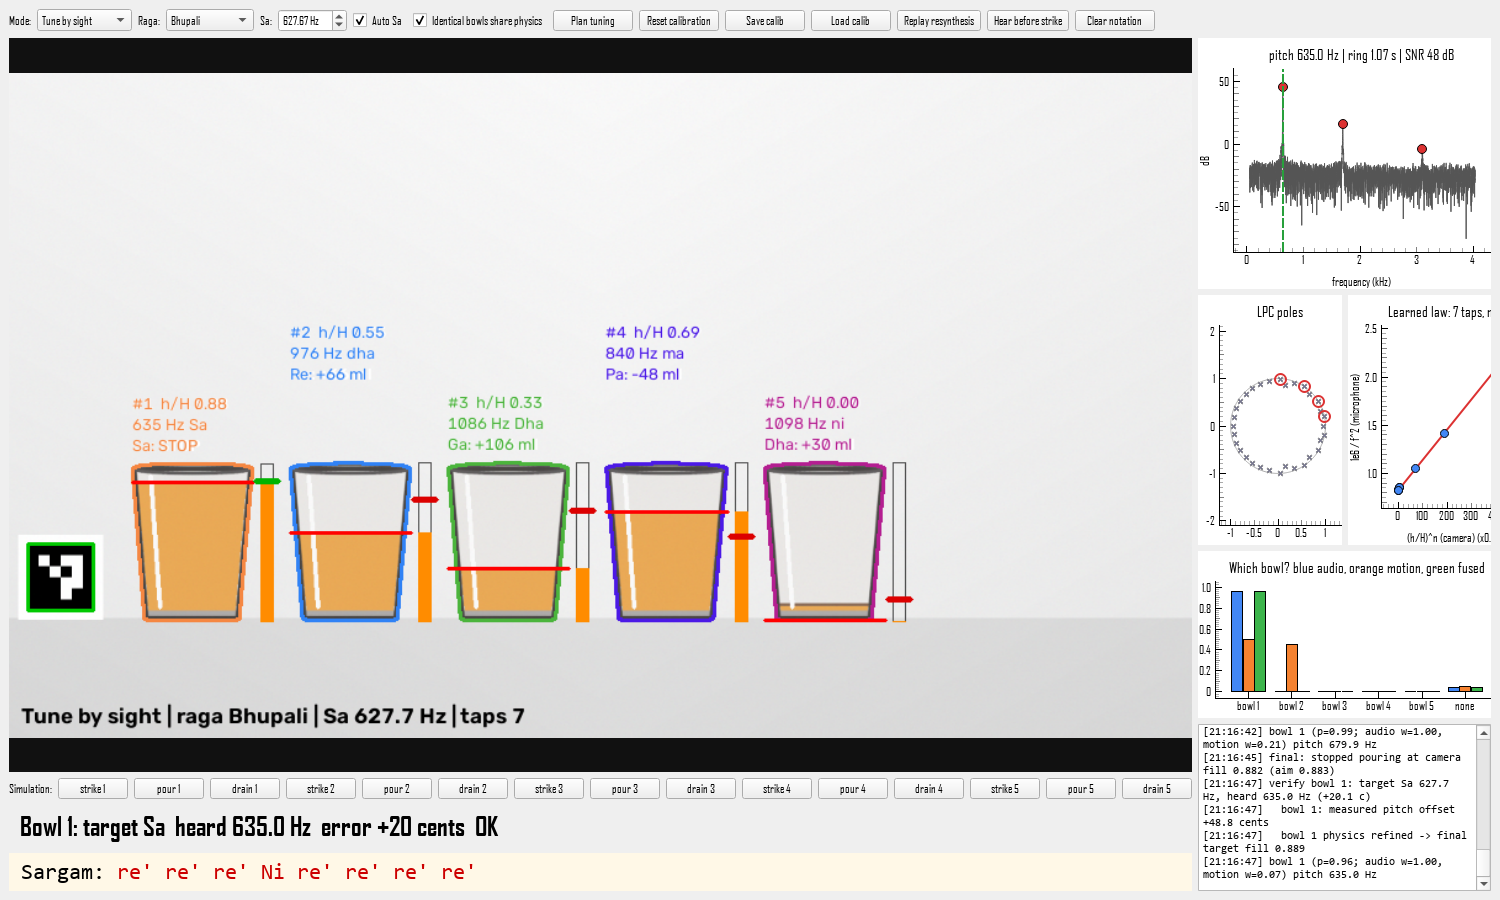
\includegraphics[width=\linewidth]{images/figures/app_screenshot.png}\par
        {\tiny Desktop app (webcam + mic, or \texttt{--sim}): water lines, targets, spectrum, LPC poles, learned law.\par}
        \vspace{2mm}
        \begin{minipage}[c]{0.52\linewidth}
            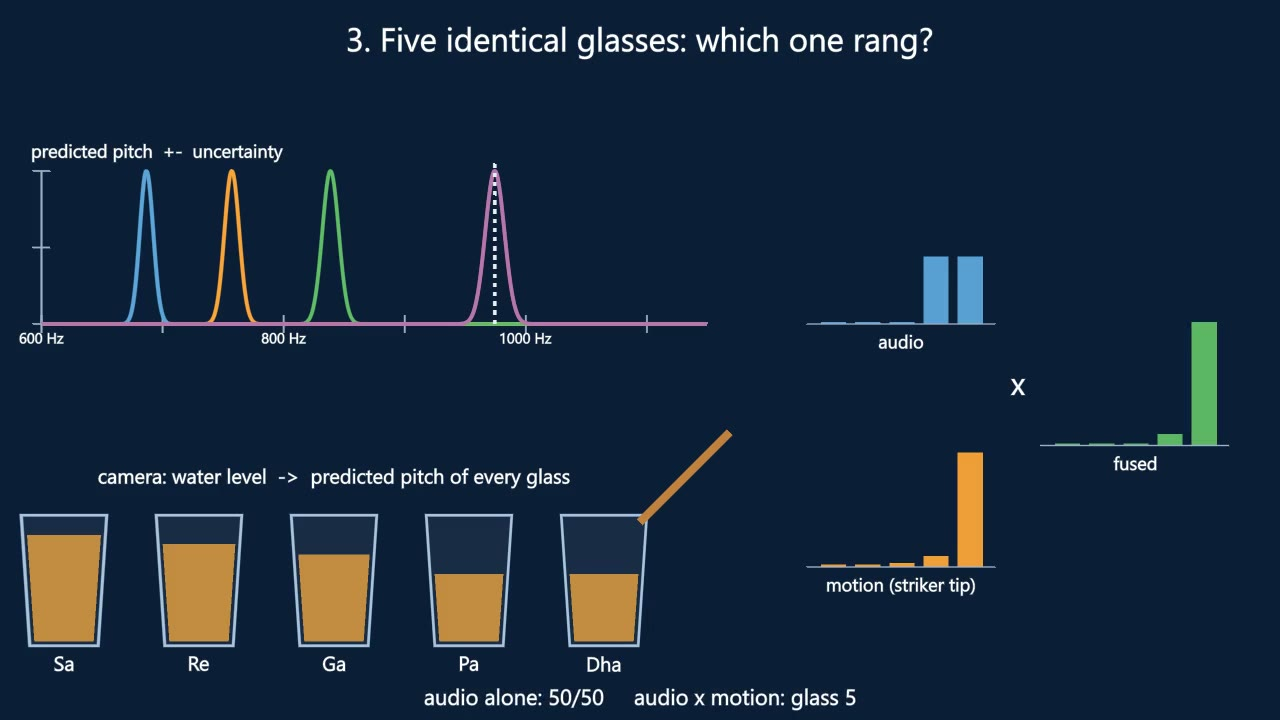
\includegraphics[width=\linewidth]{images/figures/anim_which.jpg}
        \end{minipage}\hfill
        \begin{minipage}[c]{0.45\linewidth}
            \raggedright\tiny
            Explainer page \texttt{web/index.html}: five ManimGL animations, the architecture diagram and five live in-browser demos.
        \end{minipage}
    \column{0.44\textwidth}
        \begin{exampleblock}{Conclusion}
            \scriptsize
            \begin{itemize}
                \item One physical law lets each modality predict the other.
                \item Fusion solves what neither sense can alone: identical bowls, noise, pitch ties.
                \item A few taps calibrate it; it then tunes a jal tarang by sight and writes the sargam.
            \end{itemize}
        \end{exampleblock}
        \begin{block}{Try it}
            \scriptsize
            \texttt{python app/app.py --sim}\\
            \texttt{python app/app.py} \hfill(webcam + mic)\\
            open \texttt{web/index.html}\\[2pt]
            \texttt{github.com/KUSHAGRA2606/TuneSight}
        \end{block}
    \end{columns}
\end{frame}



\section*{References}
\begin{frame}
    \frametitle{References: papers}
    \begin{multicols}{2}
    \bibliographystyle{ieeetr}
    \bibliography{ref.bib}
    \end{multicols}
\end{frame}

\begin{frame}{References: data, code, course material and tools}
    \scriptsize
    \begin{columns}[T]
    \column{0.49\textwidth}
        \textbf{Course material}
        \begin{itemize}
            \item DA321 lecture notes, IIT Guwahati: sound, images, multimodal fusion
            \item SPIN Lab interactive pages (\texttt{spinlabiitg.github.io/vip}, \texttt{/sap}): design reference for the web explainer
        \end{itemize}
        \textbf{Data}
        \begin{itemize}
            \item ObjectFolder Real: impact recordings of real objects (\texttt{objectfolder.stanford.edu}) \cite{gao2023objectfolder}
            \item Everything else: the project's physics-based simulator, with known ground truth
        \end{itemize}
        \textbf{This project}
        \begin{itemize}
            \item \texttt{github.com/KUSHAGRA2606/TuneSight}: library, desktop app, experiments, slides, web explainer
        \end{itemize}
    \column{0.49\textwidth}
        \textbf{Open-source software}
        \begin{itemize}
            \item ManimGL by 3Blue1Brown (\texttt{github.com/3b1b/manim}): the animations
            \item OpenCV (with ArUco), NumPy, SciPy, matplotlib
            \item PySide6 and pyqtgraph (desktop app); sounddevice and soundfile (audio)
            \item LaTeX Beamer with the IITG template; TikZ for every diagram
        \end{itemize}
        \textbf{LLM tools}
        \begin{itemize}
            \item Claude (Anthropic), used through Claude Code as a coding and writing assistant for the implementation, experiments,
                  figures and slides. All results were run and checked locally.
        \end{itemize}
    \end{columns}
\end{frame}

\end{document}
